% 初中衔接：精确坐标 A(0,2), B(4,6), P(2,0), M(2,4)
\begin{center}
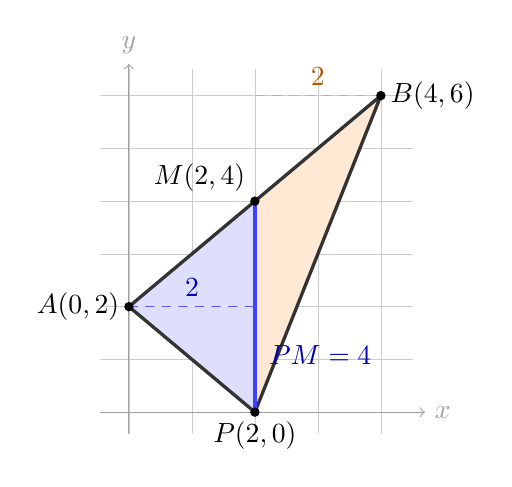
\begin{tikzpicture}[x=0.8cm,y=0.67cm, line cap=round, line join=round]
  \draw[gray!40,step=1,very thin] (-0.45,-0.4) grid (4.5,6.5);
  \draw[->,gray!75] (-0.45,0)--(4.7,0) node[right] {$x$};
  \draw[->,gray!75] (0,-0.4)--(0,6.6) node[above] {$y$};
  \coordinate (A) at (0,2);
  \coordinate (B) at (4,6);
  \coordinate (P) at (2,0);
  \coordinate (M) at (2,4);
  \fill[blue!13] (P)--(A)--(M)--cycle;
  \fill[orange!17] (P)--(M)--(B)--cycle;
  \draw[very thick,black!80] (P)--(A)--(B)--cycle;
  \draw[very thick,blue!75] (P)--(M);
  \draw[dashed,blue!65] (A)--(0,2)--(2,2);
  \draw[dashed,orange!75] (B)--(2,6);
  \fill (A) circle (1.7pt) node[left] {$A(0,2)$};
  \fill (B) circle (1.7pt) node[right] {$B(4,6)$};
  \fill (P) circle (1.7pt) node[below] {$P(2,0)$};
  \fill (M) circle (1.7pt) node[above left] {$M(2,4)$};
  \node[blue!70!black,anchor=south] at (1,2.0) {$2$};
  \node[orange!70!black,anchor=south] at (3.0,6.0) {$2$};
  \node[blue!70!black,right] at (2.07,1.08) {$PM=4$};
\end{tikzpicture}
\end{center}
